\documentclass[12pt]{book}
\usepackage{amsmath}
\usepackage{listings}
\usepackage{graphicx}


%\lstset{language=Java,basicstyle=\footnotesize,fancyvrb=true,captionpos=t}
\newcommand{\lllhome}{../../../examples/src/main/java/de/unidue/inf/is/ezdl/examples/}
\lstset{language=Java,%
	basicstyle=\scriptsize,%
	captionpos=t,%
	frame=single,%
	numbers=left,%
	rangebeginprefix=/*\ <,%
	rangebeginsuffix=>\ */,%
	rangeendprefix=/*\ </,%
	rangeendsuffix=>\ */,%
	includerangemarker=false,%
	float=b%
	}


\title{ezDL -- Developer Guide}
\author{Working Group Information Engineering, University of Duisburg-Essen}
\date{}
\begin{document}
  \maketitle 
  
\tableofcontents  

  
%%%%%%%%%%%%%%%%%%%%%%%%%%%%%%%%%%%%%%%%%%%%%%%%%%%%%%%%%%%%%%%%%%%%%%%%%%%%%%%%%%%%%%%%%
%
%
%
%
%
\chapter{Introduction}



%%%%%%%%%%%%%%%%%%%%%%%%%%%%%%%%%%%%%%%%%%%%%%%%%%%%%%%%%%%%%%%%%%%%%%%%%%%%%%%%%%%%%%%%%
%
%
%
%
%
\chapter{Building}

Before changing anything in the code, you will want to make sure that the code in your repository actually builds and passes the tests. This chapter will walk you through building the project.

EzDL is built using Maven. This offers two different options: using Maven on the command line and using it in Eclipse through a plugin. The following section introduces building using the command line. The usage of the Eclipse plugin is demonstrated afterwards.


\section{Maven on the command line}

Once you have the ezDL project checked out in your file system, you are ready to build it.

The build process is fully automated. If everything works as expected, Maven will first download resources that the build process or ezDL itself depend on (,,dependencies''). Then the system is built and tested. To start the process, open a shell (command line interface), change into the ezDL project directory and type the following\footnote{In this and the following examples, ,,\$'' is the command line's prompt and is not to be typed.}:

\begin{verbatim}
$ mvn clean install
\end{verbatim}

The process will take a few minutes---mainly because of the tests.



\section{Maven in Eclipse}

To build the project in Eclipse, the Maven plugin has first to be installed and the project has to be configured to use Maven properly. These steps, outlined in the following two sections, have only to be performed once per freshly cloned ezDL project. The build process, described in section \ref{sec:build-eclipse}, can be performed repeatedly without repeating the first steps.


\subsection{Preparations}

Install a Maven plugin for Eclipse using the ,,Install New Software'' option in the ,,Help'' menu.

Make sure that the plugin is configured to allow for nested modules. This option can be found in the Preferences under ,,Maven'' and is named ,,Support multiple Maven modules mapped to a single Eclipse workspace project''. You can use the Preferences dialog's search feature to find the option by entering a few keywords of that phrase.


\subsection{Configuring the project \label{sub:configuring}}

After installing and configuring the Maven plugin, the first step is to configure the Eclipse project to use Maven. Then we switch to nested modules and then we are ready to build. The steps are the following:

\begin{enumerate}
\item Right-click on the ezDL project and select ,,Maven$\rightarrow$Enable Dependency Management'' and wait until Eclipse is idle again.
\item Right-click on the ezDL project and select ,,Maven$\rightarrow$Enable Nested Modules'' and wait until Eclipse is idle again. This option is only visible if you previously configured Maven to allow ,,multiple Maven modules mapped ...'' as described above.
\item Right-click on the ezDL project and select ,,Maven$\rightarrow$Update Project Configuration'' and wait until Eclipse is idle again. In some cases you have to refresh the whole project and afterwards again select to ,,Update Project Configuration''. This step might take some time because Eclipse changes the layout of the project entirely and starts a build process.
\end{enumerate}


Important: The text encoding should be set so ,,UTF-8'' and the line breaks to ,,Unix'' in the properties dialog of the project.

The developers of ezDL agree on a coding style that is supposed to make the code clearly readable and independent from the taste of the individual developer. Also, this makes patches and diffs (and thus, merging) much easier.

To make formatting conforming to the coding style easier, two Eclipse configs are shipped with the project.

In the Preferences, go to ,,Java$\rightarrow$Code Style$\rightarrow$Formatter''. Click on "Import". Navigate to your project and go to the sub-directory "eclipse". Select {{{ezDL-code-formatting-ecplise.xml}}}. Then click ,,Apply''.

Next, go to ,,Java$\rightarrow$Code Style$\rightarrow$Clean Up''. Click on ,,Import''. Navigate to your project and go to the sub-directory {\tt eclipse}. Select {{{ezDL-cleanup.xml}}}. Then click ,,Apply''.

Now you can auto-format your code usign Ctrl-Shift-F and clean up by Ctrl-Shift-O.



\subsection{Building \label{sec:build-eclipse}}

To actually build the project, right-click on the project and select ,,Run As$\rightarrow$Maven install''.

Actually, there are a few different things to chose from the ,,Run As'' context menu:

\begin{description}
\item[Maven clean] will remove all generated code and binaries from the Maven project.
\item[Maven package] will build the whole project and test it but omit certain checks.
\item[Maven install] will perform several checks (e.g. for the right license headers in each .java-File), build the whole project and test it.
\end{description}

When things look dicey and you want to be sure that there aren't any old binaries interfering with your new changes, you should perform a ,,Maven clean'' before proceeding with the build.

There are versions of the Maven plugin that are not very well integrated into Eclipse. This may lead to problems after building the Maven project such as classes or resources not being found when starting test cases right out of Eclipse (e.g. using ,,Run as$\rightarrow$JUnit Test''). In these situations you should rebuild the project in Ecplise, too, using the options provided by the ,,Project'' menu in Eclipse. This can be done by switching to auto-building the project (this is the default) and performing a clean, resulting in an automatical rebuild. After this you should be able to run and debug the code in Eclipse.



%%%%%%%%%%%%%%%%%%%%%%%%%%%%%%%%%%%%%%%%%%%%%%%%%%%%%%%%%%%%%%%%%%%%%%%%%%%%%%%%%%%%%%%%%
%
%
%
%
%
\chapter{How we code}

Please be aware that there are two target audiences for your code. The one that probably first comes to mind is the compiler since code is the only way to communicate with it. The compiler's requirements concerning the code are very strictly defined but easy to follow: the syntax has to be right. The compiler doesn't care about much more. The second target audience, though, is much harder to write for: it's the next guy responsible for maintaining your code. This guy can also easily be yourself. Especially in long-term programming efforts like ezDL programmers frequently revisit their own code months after writing it and get angry at the stupid person how wrote that illegible piece of nonsense. The only way to get around that is writing for two target audiences at once: the compiler and human beings that have no  knowledge about the code and the rationale behind it for what ever reason. This means that on the one hand code should communicate clearly what it is supposed to do and obey a common writing style to reduce the noise that would arise if each programmer used only her own sense of elegance.

Therefore, just about every software project has its own style of how code is written---that is, if you count total chaos as a style. In ezDL we have a set of formatting rules and some writing guidelines we try to follow. The formatting rules are stored in an Eclipse config file file that is shipped with the project. See section \ref{sub:configuring} for details. The question how the code should communicate with fellow developers are higher-level guidelines that cannot be externalized to a file very well. This has two consequences: One is that there is (currently) no way to automatically transform badly written code to good code. The other one is that there is also (currently) no good way to automatically recognize either bad or good code. 

That means that on the other hand programmers have to follow some rules when writing the code and that other programmers have to make sure that the code complies to the standards. But what exactly are those standards? We try to summarize them in this chapter by starting with badly written pieces of code and show how to improve them so they would pass a code review.






\section{Write self-documenting code}

Every programmer loves self-documenting code because if the code documents itself the programmer doesn't have to. Right? Wrong. Self-documenting code is not code that the reader has to figure out by herself. ``Self-documenting'' means that the programmer uses techniques to document the way the code works that exclude inline comments. 

Inline comments are sometimes used when code isn't really obvious at first glacen. Like this:

\begin{lstlisting}[caption=selfdoc1.java] 
public Object getStructure(Document document, Map<String, Object> props) {
    ...
    int cmp = input.length();
    if (cmp > 10000) {
        System.out.println("This page is very large. Structuring " 
          + "will take at least " + ((cmp / 10000)) + " minutes!!!");
    }
    input = input.replaceAll("<!--.*?-->", ""); // remove all comments!
    String part1 = "";
    String part2 = "start!";

    // process the input
    while ((!input.equals("")) && (counter < 40) && (!part2.equals("")) 
       && (shift >= 0)) {
        ...
    }
    ...
}
\end{lstlisting}

This code is taken from an early version of {\tt ToolkitAPI.java}. Several questions arise that should be addressed. And some questions are already answered by using inline comments. Some open questions are:

\begin{itemize}
\item What happens to {\tt cmp} later?
\item What does the {\tt 10000} mean? Why isn't 3 used? Or 10000000? 
\item What do {\tt part1} and {\tt part2} hold? What object are these part of?
\item What do the 80 lines of code (with lots of nested {\tt if} and {\tt for}) in the {\tt while} loop do? To what input? What is the output?
\end{itemize} 

Inspecting the code we find out that {\tt cmp} is only used in comparisons (thus the name, we guess) as a shorthand for {\tt input.length()}. So we rename the variable properly and use the {\tt final} modifier tosignify that the variable is never modified\footnote{The {\tt final} modifier is used to make the code clearer. It also saves a few CPU cycles under certain conditions but this is just a nice side-effect here. The following steps towards better legibility make the code less efficient---e.g. by computing things that might not be needed. So there is a trade-off between legibility and performance. To quote Donald E. Knuth: ``Premature optimization is the root of all evil''. You should first make sure that your code can be maintained und bug-fixed easily. The standard here is both other programmers and you in three months. If the code seems correct but slow, look for performance bottlenecks and optimize them when you know where they are. Just optimizing stuff to death that might be executed only twice per decade doesn't help performance-wise and makes the code less easy to understand.}:

\begin{lstlisting}[caption=selfdoc2a.java] 
    final int inputLength = input.length();
    if (inputLength > 10000) {
        System.out.println("This page is very large. Structuring "
          + "will take at least " + ((inputLength / 10000)) + " minutes!!!");
    }
\end{lstlisting}

Now we address the {\tt 10000}. Analyzing the output, the 10000 might be a constant with the dimension $min^{-1}$, holding how many characters of input per minute the code can process. Since this value is fixed, we give it a name and use it:


\begin{lstlisting}[caption=selfdoc2b.java] 
    final int inputLength = input.length();
    final int charsPerMinute = 10000;
    if (inputLength > charsPerMinute) {
        System.out.println("This page is very large. Structuring "
          + "will take at least " + ((inputLength / charsPerMinute)) 
          + " minutes!!!");
    }
}
\end{lstlisting}

Please note that this code still has the problem of having the speed wrong on most machines. If the estimate was really important, you would want to calculate the speed first.

But the code is still not well documented. The comparison in the {\tt if} clause is strange. The input size is compared to a speed. That doesn't sound right. What is meant instead, is to calculate how many minutes the code needs to process the input. If that time is longer that a minute, the warning should be printed. We notice that this calculation is actually done later in the {\tt println} statement. So we reformulate the code a bit to get it right:


\begin{lstlisting}[caption=selfdoc2c.java] 
    final int inputLength = input.length();
    final int charsPerMinute = 10000;
    final int processingTimeMinutes = inputLength / charsPerMinute;
    if (processingTimeMinutes >= 1) {
        System.out.println("This page is very large. Structuring "
          + "will take at least " + processingTimeMinutes) + " minutes!!!");
    }
}
\end{lstlisting}

The name of the new final variable, {\tt processingTimeMinutes} combines a name for the content and the unit of the value. If {\tt Minutes} was omitted here, the reader would have to analyze the code in order to find out if the calculation is about seconds, minutes, hours, days or years. It is a good habit to use the unit as a part of the name of a variable---especially for private static fields.

On to the next snippet:

\begin{lstlisting}[caption=selfdoc3a.java] 
public Object getStructure(Document document, Map<String, Object> props) {
    ...
    input = input.replaceAll("<!--.*?-->", ""); // remove all comments!
    ...
}
\end{lstlisting}

Nice comment. But what if the programmer later finds out that this doesn't suffice to remove all comments?


\begin{lstlisting}[caption=selfdoc3b.java] 
public Object getStructure(Document document, Map<String, Object> props) {
    ...
    input = input.replaceAll("<!--.*?-->", ""); // remove all comments!
    input = input.replaceAll("^//.*$", ""); // remove line comments!
    ...
}
\end{lstlisting}

And it gets uglier. Unless the code is really time-critical a nicer way to do it is this:

\begin{lstlisting}[caption=selfdoc3c.java] 
public Object getStructure(Document document, Map<String, Object> props) {
    ...
    input = removeAllComments(input);
    ...
}

String removeAllComments(String input) {
    input = input.replaceAll("<!--.*?-->", ""); // remove all comments!
    input = input.replaceAll("^//.*$", ""); // remove line comments!
    return input;
}
\end{lstlisting}

Now, reading {\tt getStructure()} is easier. It is clear that comments are removed from the input but the exact way is no longer important. Please note that the new method, {\tt removeAllComments()}, is package visable to help with unit testing but not public since it is not part of the outside view of what the object does. 

The code can be further restructured if the inline comments in {\\tt removeAllComments} are not wanted:

\begin{lstlisting}[caption=selfdoc3c.java] 
String removeAllComments(String input) {
    input = removeXMLComments(input);
    input = removeLineComments(input);
    return input;
}

String removeXMLComments(String input) {
    input = input.replaceAll("<!--.*?-->", "");
    return input;
}

String removeLineComments(String input) {
    input = input.replaceAll("^//.*$", "");
    return input;
}
\end{lstlisting}


What is nice about these new methods is: they can both be tested separately and they can be commented on the method level, giving information on the inputs and outputs and maybe preconditions and postconditions. Using commented methods also shows the scope of the comments. If there are 100 lines of spaghetti code with a comment like ``calculate foo'' at line 20, nobody would know how many lines are needed to calculate foo, unless the following code is analyzed further. Moving the calculation to a new method and commenting it makes it all clearer and the calculation is even reusable in other methods of the class. This kind of JavaDoc is also way better supported by IDEs such as Eclipse.

There is another part up for being edited:

\begin{lstlisting}[caption=selfdoc4a.java] 
public Object getStructure(Document document, Map<String, Object> props) {
    ...
    // process the input
    while ((!input.equals("")) && (counter < 40) && (!part2.equals("")) 
      && (shift >= 0)) {
        ...
    }
    ...
}
\end{lstlisting}

The while loop. As mentioned above, the code inside the while loop is 80 lines long and deeply nested. 80 lines of nested code is often a warning signal. The whole while loop should be moved into a new method that has a name that documents what the loop actually does. But even then we have a problem: the condition in the while loop is not easy to get. What does it mean that input equals the empty string?  Why should counter stay below 40? Why not 42? And so on. 

To get around that, we can use the above tactic of giving literals symbolic names and rename variables so that it is clear what they are about.

\begin{lstlisting}[caption=selfdoc4a.java] 
public Object getStructure(Document document, Map<String, Object> props) {
    ...
    // process the input
    final int maxIterations = 40;
    final int minNestingLevel = 0;
    while ((!input.equals("")) 
      && (iterations < maxIterations) 
      && (!part2.equals("")) 
      && (nestingLevel >= minNestingLevel)) {
        ...
    }
    ...
}
\end{lstlisting}

If loop conditions are too complex, it might be better to refactor the whole condition into a new method and document the method. Sometimes, a complex loop condition is a sign for the loop being improvable by simplification.

At this point we still don't know about the reasons for the parts of the conditions that compare against the empty string\footnote{something that should be done with at least {\tt String.length()} or better {\tt String.isEmpty()} depending on the Java version} but we leave that as an exercise to the reader.



\subsection{Guidelines}

After giving some examples on how to solve particular problems, we'd like to give you a list of guidelines that should lead to more comprehensible code.

\begin{description}
\item[Use sensible names.] This starts with using nouns for classes and verbs for methods. It also means that variable names such as ``foo'' and ``bar'' or ``i'' should be avoided even if they show that you probably know your fair share of hacker culture. Variables like ``i'' can be used in {\tt for} loops if it is absolutely clear what the variable stores. When choosing a variable name, try to make sure that the name you're going to use is actually a good representation of the named entity. E.g. a method that adds an item to a list as long as that item has a certain property (like not being null) should not be named {\tt add} because the user might believe that also null references can be added. A name like {\tt addIfNotNull} is much clearer, if longer, and leads to fewer misunderstandings when it comes to corner cases of input. Other examples for bad naming are {\tt getDate} when the method returns a string representation of a date and {\tt ..}
\item[Use methods instead of commented code blocks.] If you have a long method that performs several steps on some input, consider breaking the steps down into new private methods and call them. That way you can get around commenting code (with the inherent ambiguity of not saying where the code stops that the comment is about) and have a clearly defined interface.
\item[Make sure each entity is about exactly one thing.] Classes should deal with one entity or one kind of behaviour. Having classes perform different things like searching for documents and retrieving document details depending on a part of the input is difficult. It's difficult to read because the class might get large, it's difficult to extend, it's difficult to remove behaviour because nobody knows which properties are affected and so on. Instead write one class to search and one class for the detail retrieval. If you don't need the detail retrieval (or want to experiment with a different way to do it) you can delete the class or rewrite it.
\end{description}








%%%%%%%%%%%%%%%%%%%%%%%%%%%%%%%%%%%%%%%%%%%%%%%%%%%%%%%%%%%%%%%%%%%%%%%%%%%%%%%%%%%%%%%%%
%
%
%
%
%
\chapter{Architecture}

The architecture aims for good object-oriented design. Part of that goal is the decoupling of components. In ezDL this is done by using message passing for communication between larger components (e.g. between agents in the back end or between the client and the back end) and even between smaller ones (like tools in the front end). See figure \ref{fig:systemarchitecture} for a diagram of the top-level view. On the right side there is the back end that does the grunt work in ezDL like searching remote digital libraries for documents. On the left side is a client application that communicates with the back end through a Message Transfer Agent (MTA). An MTA serves as an interface between clients and the back end and hides the inner workings of the back end from the client. A client asks the MTA for documents that have ``algorithm'' in the title and the MTA answers with a list of such documents. How the MTA does that is not of interest to the client. 

How the back end performs the tasks (currently) can be seen in figure \ref{fig:backendarchitecture}. On the left are the MTAs that make the system border. The long box at the bottom is a communications infrastructure like a CORBA ORB or a JMS broker. The other boxes are agents. Agents are software systems each of which runs in their own JVM and is responsible for one well-defined thing or family of things. The user agent, e.g., is the place where information about users is stored: their login credentials, their preferences, and so on. The search agents searches, the repository agent stored documents and the query history agent stores query histories. The directory agent is special because it facilitates communication between agents by knowing which agents are available and what kind of service they offer. Agents can ask the directory for the name of an agent that offers a specific service. This is the reason why starting the back end is performed in the following order:

\begin{enumerate}
\item Communication infrastructure (e.g. JMS broker)
\item Directory
\item Agents and wrappers
\item MTA's
\end{enumerate}

The MTA's are started last because otherwise they would offer an interface to a system that is not yet ready for serving requests.


\begin{figure}[t]
\begin{center}
  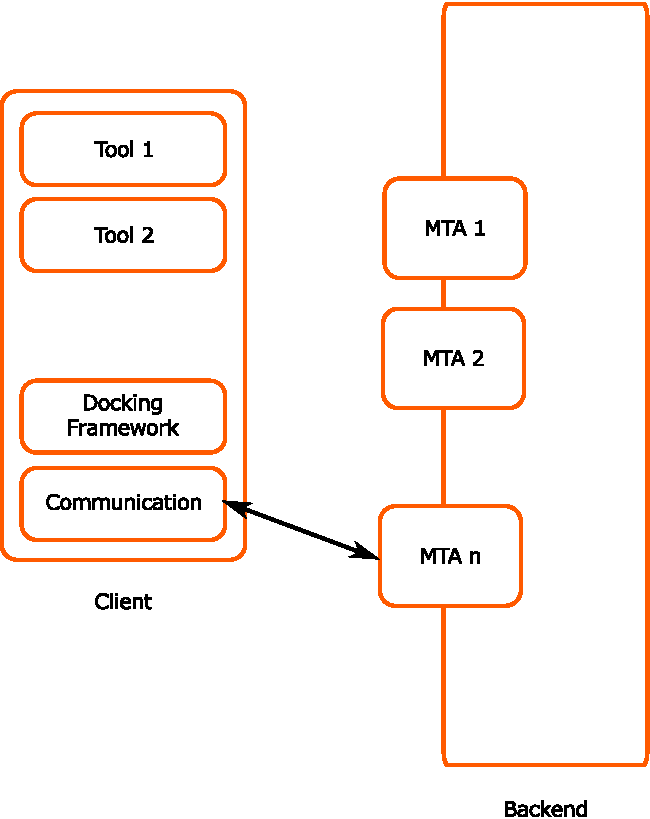
\includegraphics[width=.75\linewidth]{system-architecture}
  \caption[The high-level architecture]{The architecture of ezDL on the highest level}
  \label{fig:systemarchitecture}
\end{center}
\end{figure}

\begin{figure}[t]
\begin{center}
  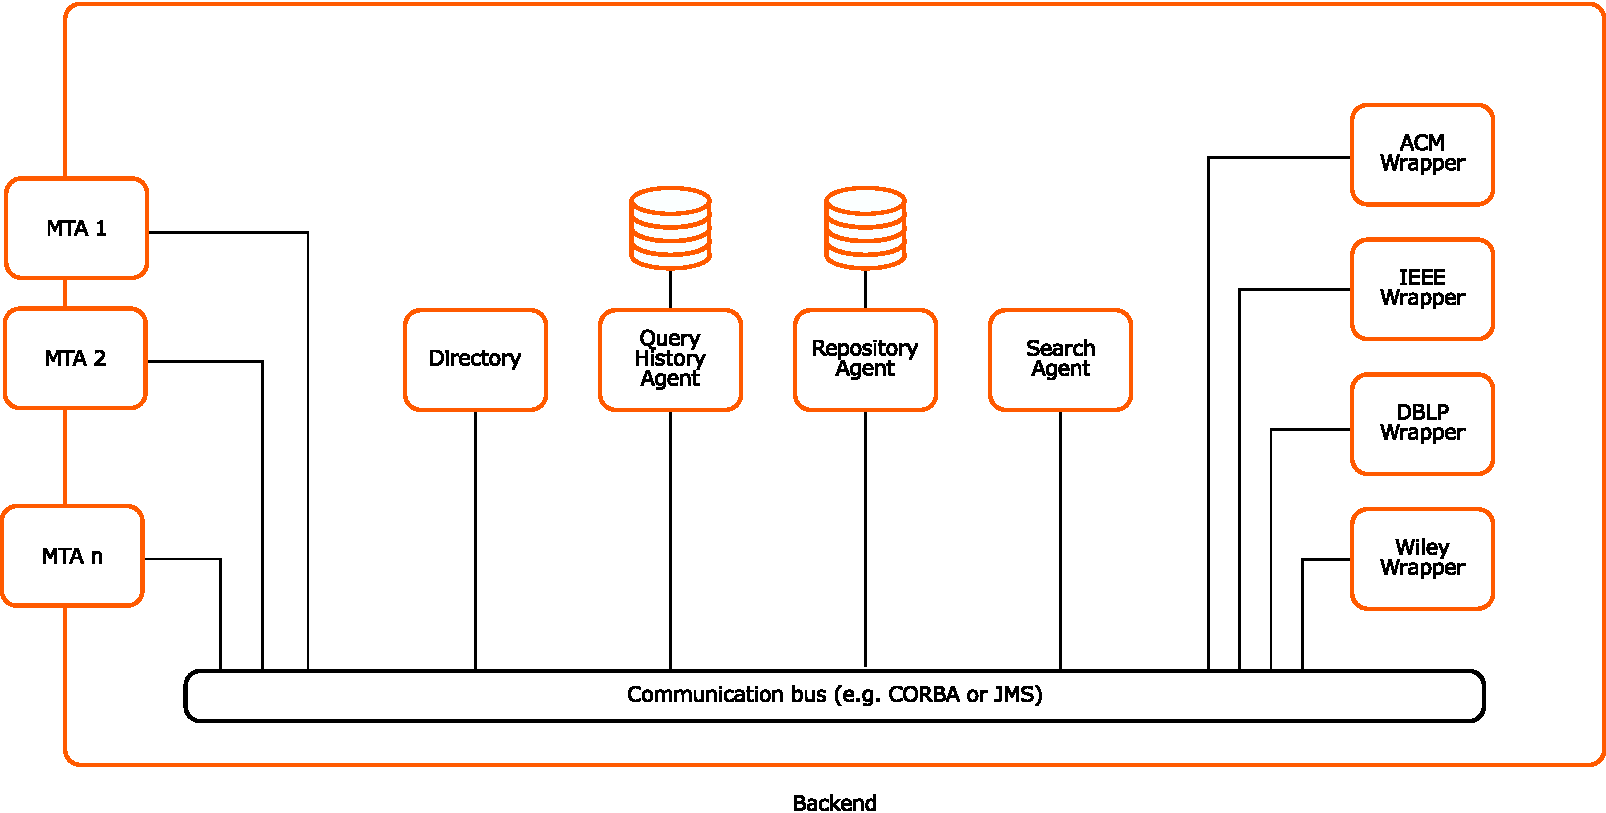
\includegraphics[width=.75\linewidth]{backend-architecture}
  \caption[The back end architecture]{The architecture of the ezDL back end}
  \label{fig:backendarchitecture}
\end{center}
\end{figure}





%%%%%%%%%%%%%%%%%%%%%%%%%%%%%%%%%%%%%%%%%%%%%%%%%%%%%%%%%%%%%%%%%%%%%%%%%%%%%%%%%%%%%%%%%
%
%
%
%
%
\chapter{Agents \label{ch:agents}}

\section{General architecture \label{sec:agents:architecture}}

\begin{figure}[t]
\begin{center}
  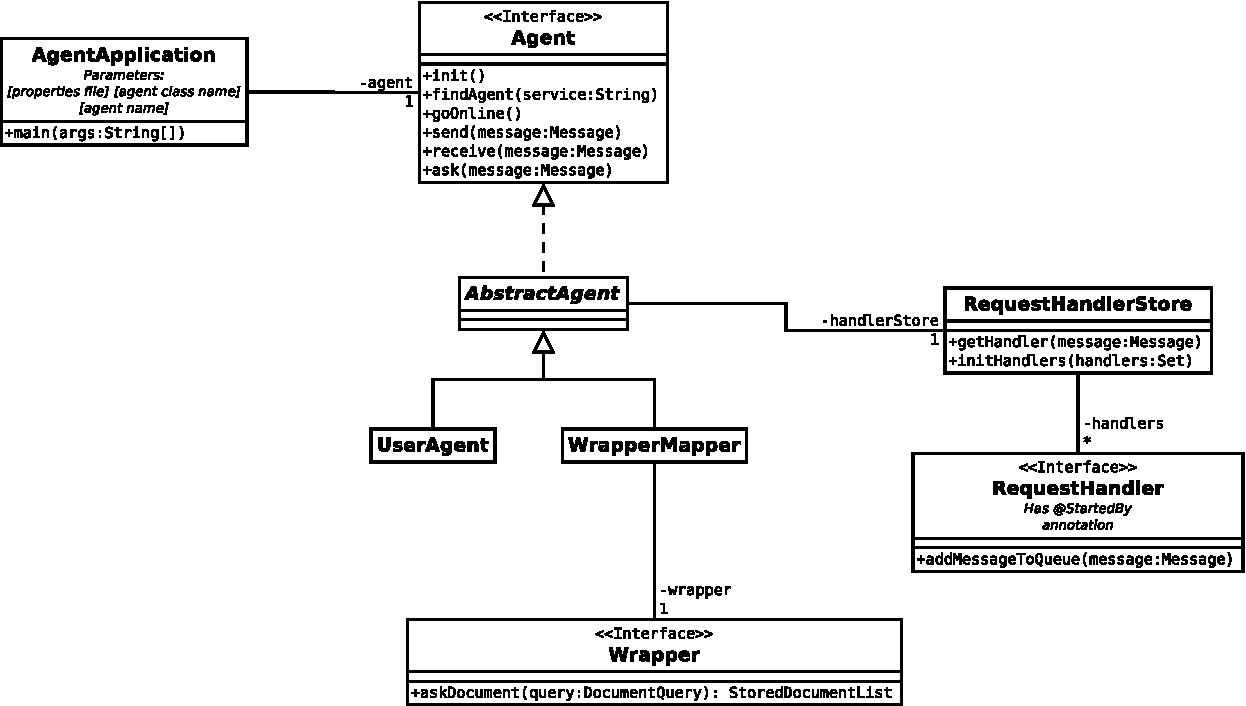
\includegraphics[width=.75\linewidth]{Agent}
  \caption{The architecture of an Agent}
  \label{fig:agentarchitecture}
\end{center}
\end{figure}



The active components in the back end  operate as agents, meaning they are processes that communicate witch each other to fulfill their tasks. The communication is realized using a common mechanism that is beyond the scope of this section and, basically, beyond the scope of the agents themselves because the communication is hidden behind interfaces. This allows developers and operators to use the middleware that suits them best. Available and implemented middlewares are CORBA and ActiveMq.

The first thing an agent does when it is started is registering with the directory. The directory is a central agent that knows about all the other agents and their capabilities. 

The registration message contains the name of the agent, the name of the service that it implements and possibly more information. If the agent is a wrapper (see chapter \ref{ch:wrappers}), the registration also contains information about the wrapped remote site and performance metrics.

The service that an agent implements is the kind of action that it performs. The service names are structured hierarchically in the form of UNIX directory names. E.g. all common services are under {\tt /service} and wrappers are under {\tt /wrapper}. Wrappers that wrap digital libraries are under {\tt /wrapper/dl} and so on.

See figure \ref{fig:agentarchitecture} for an overview of some subcomponents of agents. At the top is the {\tt Agent} interface that every agent has to implement. Below that is the {\tt AbstractAgent}, a default implementation of the core behaviour of agents. {\tt AbstractAgent} implements basically everything but ``production behaviour''. It takes care of registering with the directory agent, handles incoming messages, sends messages, caches information about agent names and so on. The one thing that the {\tt AbstractAgent} does not know how to do is actually handle specific messages. Messages are handles by {\tt RequestHandler} implementors. See figure \ref{fig:requesthandlerarchitecture} for more details.

The class in the upper left corner is {\tt AgentApplication}, a helper class that has a {\tt main} method and, thus, can actually be run. {\tt AgentApplication} takes care of reading properties files and instantiating an agent class.

An agent (read: {\tt AgentApplication} with an {\tt Agent} in it) can be started multiple times as long as the names of all instances are unique. It is, e.g., possible to start multiple instances of the search agent using names like {\tt SearchAgent1} and {\tt SearchAgent2}. Since the service name is hard coded in the source of the search agent (because the service type only changes if the source is changed dramatically), all instances will be found under {\tt /service/search}. A client can then ask the directory agent for all names of agents that implement {\tt /service/search} or get just one (load-balanced) name.

Agents can use the method {\tt findAgent(String service)} to get a name of an agent that implements the given service.

There is only one agent that doesn't implement a service and whose name cannot be resolved using the directory agent: it's the directory agent itself. The name of the directory agent is configured using the properties files and can be determined in an agent by calling {\tt getDirectoryName()}.




\section{Requests and request handlers}

In ezDL, a request is a thing that some entity in the system (the user, the client, some agent) wants to get done. Entities communicate requests by sending messages to remote parties. The receiver uses a {\tt RequestHandler} to handle the request. As explained in section \ref{sec:agents:architecture}, this is done by implementing the {\tt RequestHandler} interface. Figure \ref{fig:requesthandlerarchitecture} shows more details about the relationship between agents and request handlers. It also shows that there is an {\tt AbstractRequestHandler} that can be used for implementing a request handler. The {\tt AbstractRequestHandler} takes care of all the mundane aspects of handling requests and lets the developer concentrate on actually handling the request.


\begin{figure}[t]
\begin{center}
  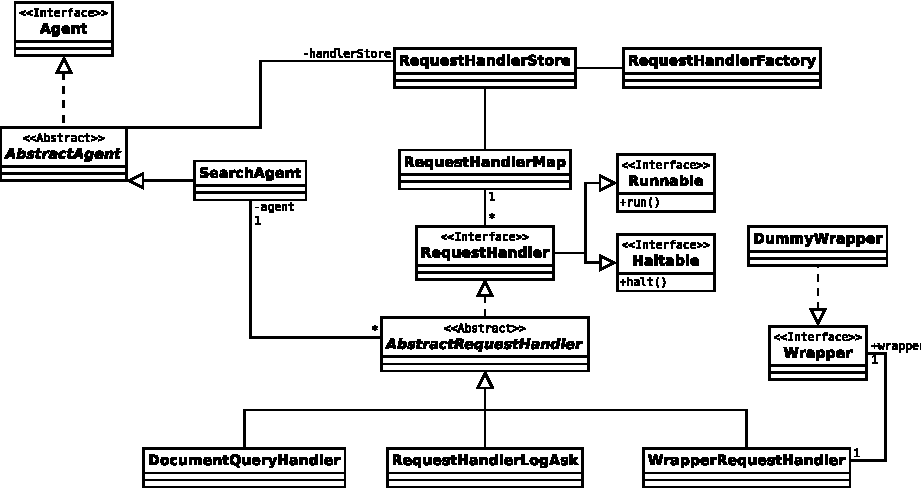
\includegraphics[width=.75\linewidth]{RequestHandlers}
  \caption{The architecture of RequestHandler}
  \label{fig:requesthandlerarchitecture}
\end{center}
\end{figure}

Request handlers are announced to the {\tt RequestHandlerStore} by the {\tt AbstractAgent}. The only thing the agent implementor has to do is override the method {\tt Agent.setupRequestHandlers()} to return a list of request handlers that should be used. The default implementation already returns a number of handlers for common things like responding to status requests so the super implementation should be called. 

The {\tt RequestHandlerStore} has to know how to deal with a given request handler. Since it only gets the class names of request handlers it should take care of, the classes have to annotated. There is one annotation that is mandatory since it tells the store which message content types the handler actually handles. The other one is optional.

\begin{description}
\item[{\tt StartedBy}] is the mandatory annotation the store uses to determine which request handler class can be used to handle an incoming message content object. It can be used like this: {\tt StartedBy(AliveAsk.class)}.
\item[{\tt Reusable}] is the optional annotation that marks a class as being thread safe. If a request handler is thread safe, it can handle multiple requests concurrently in the same object. In this case the store does not have to create a new object for each incoming message but can reuse an existing object. Request handlers that are not thread safe must not be marked by this annotation. This way each incoming message is handled by a freshly created request handler that can use internal state to deal with more complex protocols like sending messages itself and waiting for answers in order to process the request.
\end{description}

If the request handler store handles an incoming message, it first checks if the message is about a request that is already being handled by an existing request handler. Maybe the request handler sent a message to another agent and now waits for the result. To decide this, the request ID in the message is used: request handlers are tracked by the ID of the request they are processing. So if a request handler has to talk to another agent, it should use the ID of the current request for the new message so answers are routed to the request handler that sent the request. If a new request ID were used, the remote agent would answer correctly. The agent, though, would get a Tell message (e.g. {\tt DocumentDetailsTell}. It would ask the store to find a request handler for that request. Since no handler is there to handle answers (for obvious reasons) it would check if an existing request handler is running for the same request. The request ID of the incoming message being different, no existing request handler can be found and the message is finally dropped.



\section{Implementing an agent that handles a request}

As outlined in the previous sections, implementing a new agent is a two step process: first the agent has to be implemented and then the request handler has to be implemented. Listings \ref{lst:agent} and \ref{lst:reqh} show the code to get a working dummy agent that lacks any but the standard functions. In the example, the agent is implemented to announce {\tt /service/dummy} to be the service it offers and to process {\tt DummyAsk} messages by sending a {\tt DummyTell} to the sender. Please note that the request handler is marked reusable by the second annotation.


\lstinputlisting[linerange=class,label=lst:agent,caption=DummyAgent.java]{\lllhome agent/DummyAgent.java}

\lstinputlisting[linerange=class,label=lst:reqh,caption=DummyRequestHandler.java]{\lllhome agent/DummyRequestHandler.java}









%%%%%%%%%%%%%%%%%%%%%%%%%%%%%%%%%%%%%%%%%%%%%%%%%%%%%%%%%%%%%%%%%%%%%%%%%%%%%%%%%%%%%%%%%
%
%
%
%
%
\chapter{Wrappers \label{ch:wrappers}}

\section{General architecture}  
  
\section{Solr wrappers}  

\section{Toolkit wrappers}
  
  
\section{Things your new wrapper should support}

\begin{itemize}
\item search for year ranges (e.g. 2000-2009)
\item use the Filter class for post-hoc filtering incoming results from the digital library
\end{itemize}
 
 
 
\section{How to implement a new Toolkit wrapper}

Create new class that implements AbstractBasicToolkitWrapper.

Create a new test class in the test module. The test class inherits from ToolkitWrapperTestBase.

Implement methods.










%%%%%%%%%%%%%%%%%%%%%%%%%%%%%%%%%%%%%%%%%%%%%%%%%%%%%%%%%%%%%%%%%%%%%%%%%%%%%%%%%%%%%%%%%
%
%
%
%
%
\chapter{Communication}

Communication between components and subcomponents in ezDL is done by passing messages around. This chapter introduces basic concepts and explains the message content types.




\section{Messages\label{sec:communication:messages}}

Messages are used to pass information in three different contexts:

\begin{itemize}
\item between tools in the front end
\item between front end and back end
\item between agents in the back end
\end{itemize}

In each of these contexts, addressing works differently. For this reason, there are three different message types available. 

A message type acts as an envelope for The Actual Message Content. Actual message contents are stored in classes that implement the {\tt MessageContent} interface, which is merely a tagging interface.

\begin{figure}[t]
\begin{center}
  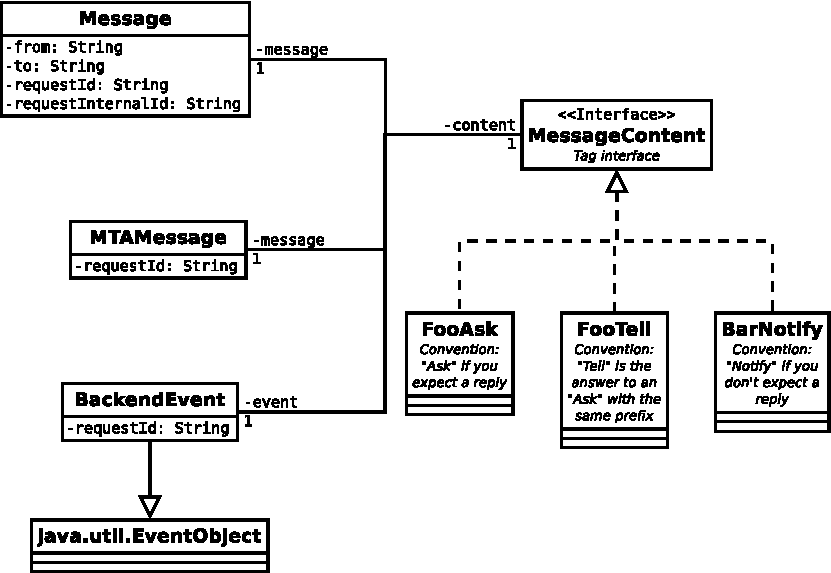
\includegraphics[width=.75\linewidth]{Message}
  \caption{The architecture of messages}
  \label{fig:messagearchitecture}
\end{center}
\end{figure}


Figure \ref{fig:messagearchitecture} shows how the various message and message content types are interconnected.

\begin{description}
\item[BackendEvent] is one of the events used by tools in the front end to communicate with each other. A BackendEvent is fired if a tool wants to communicate with the back end.
\item[MTAMessage] is the envelope that is used by the communication component in the front end to communicate with the back end. The name comes from the MTA (Message Transfer Agent) that is involved in the communication. Since front end and back end are connected using a 1:1 connection (currently a TCP connection), both sender and receiver are known and don't have to be specified. This makes sure that no conflicts can arise between the known parties on both ends of the connection and the specified parties.
\item[Message] is the envelope used by back end agents to communicate with each other.
\end{description}

Each of these envelope classes contain a {\tt MessageContent} implementor that holds the actual message payload. Decoupling the payload from the addressing also helps with repackaging payloads between system borders---e.g. in the MTA that gets an {\tt MTAMessage} object from the client and has to forward the payload using a {\tt Message} object.




\section{Message content types}

There are lots of {\tt MessageContent} types in ezDL. To make the protocols they are used in clearer, a naming convention is used. At the end of the class names either Ask, Tell or Notify are suffixed.

\begin{description}
\item[Ask] is the suffix that indicates that a content of this type implies an answer to be requested. E.g. {\tt AliveAsk}, the question ``are you still there?'' should be answered using a class {\tt AliveTell} (see below under ``tell'').
\item[Tell] is the suffix used for an answer to an Ask message content using the same prefix. E.g. a content type {\tt DocumentDetailsTell} is the answer to {\tt DocumentDetailsAsk}.
\item[Notify] is used to suffix message content types that are just sent in an FYI manner---no answer needed. Examples are {\tt CancelRequestNotify}. The intent is to tell the remote party to stop working on a request because the answer is not needed anymore, so no answer is expected.
\end{description}

Even though this is just a naming convention it is strongly recommended to follow it.





\section{Infrastructure}

How are messages transferred?



\section{The important role of the MTA in the communication between client and back end}

The client only communicates with the MTA. So the MTA has the responsibility to deal with incoming requests. This implies that new kinds of requests (e.g. the {\tt DummyAsk} used in the examples in this documentation) have to have a representation in all MTA's that are supposed to act on that request.

In the {\tt AbstractGatedMTA} there is a method that deals with forwarding incoming message content objects to agents. You'll find the first few lines in listing \ref{lst:mtatransform}. One way of making sure your new message content type is forwarded to the right agent is to add a new {\tt if} clause using the others as as a template as seen in the last few lines of the listing.

\lstinputlisting[linerange=snip,label=lst:mtatransform,caption=The transform() method in GatedHttpMTA.java]{\lllhome mta/DummyMTA.java}



\section{Communicators}




%%%%%%%%%%%%%%%%%%%%%%%%%%%%%%%%%%%%%%%%%%%%%%%%%%%%%%%%%%%%%%%%%%%%%%%%%%%%%%%%%%%%%%%%%
%
%
%
%
%
\chapter{User client}

\section{Tools}

From the user's point of view, tools are collections of views (sub-windows) that perform specific tasks. Every tool has at least one view because a view is needed to interface with the user. Tools can have many views. The search tool, e.g. has the search form view, the library choice view and the result view.


\section{Implementing a tool}

In order to implement a tool that the user can interact with, two interfaces have to be implemented: {\tt Tool} and {\tt ToolView}. To speed up the development process, abstract implementations of these interfaces are available. See figure \ref{fig:toolarchitecture} for an overview of the architecture of tools and listings \ref{lst:tool} and \ref{lst:toolview} for minimalistic sample implementations.

The code in listing \ref{lst:toolview} creates a new view that has a button with the label ``test'' in it. 

The code in listing \ref{lst:tool} creates a tool that uses the {\tt DummyToolView}. It does not, though, react to events. If event were to be handled, the method {\tt handleEzEvent(EventObject)} had to be implemented accordingly.



\lstinputlisting[linerange=class,label=lst:tool,caption=DummyTool.java]{\lllhome tool/DummyTool.java}

\lstinputlisting[linerange=class,label=lst:toolview,caption=DummyToolView.java]{\lllhome tool/DummyToolView.java}


\begin{figure}[t]
\begin{center}
  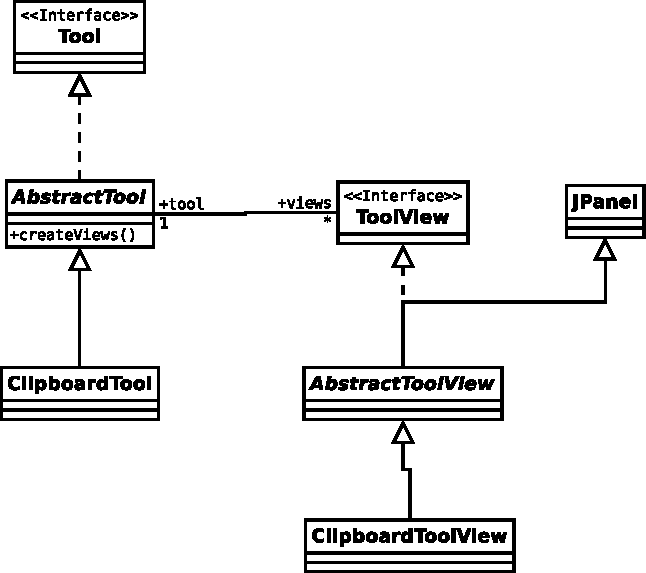
\includegraphics[width=.75\linewidth]{Tool}
  \caption{The architecture of tools}
  \label{fig:toolarchitecture}
\end{center}
\end{figure}

In the state listed here, the tool and view don't do anything but sit there. 

In order to have the button send a message to the backend we have to implement a suitable message content type. See listing \ref{lst:content} for a very boring content type.

\lstinputlisting[linerange=class,label=lst:content,caption=DummyAsk.java]{\lllhome agent/DummyAsk.java}


We can edit the view to make it send a message to the back end when the button is pressed. See listing \ref{lst:toolviewmessage} for details.

\lstinputlisting[linerange=class,label=lst:toolviewmessage,caption=SendingToolView.java that sends a message]{\lllhome tool/SendingToolView.java}




%%%%%%%%%%%%%%%%%%%%%%%%%%%%%%%%%%%%%%%%%%%%%%%%%%%%%%%%%%%%%%%%%%%%%%%%%%%%%%%%%%%%%%%%%
%
%
%
%
%
\chapter{Human Interface Guidelines}

The Human Interface Guidelines describe the structure of the elements of the ezDL user interface and common patterns of interaction.

All specifications regarding positions refer to LTR languages (e.g. English). If RTL languages (e.g. Arabic) is to be implemented in ezDL, these specifications have to be adapted according to the conventions used in the target language.


Links:
\begin{itemize}
\item http://www.qalabs.com/resources/newsletters/archive/newsletter37.htm
\item http://library.gnome.org/devel/hig-book/stable/index.html.en - Gnome HIG 2.2
\item http://wiki.openusability.org/guidelines/ - KDE HIG
\item \item http://msdn.microsoft.com/en-us/library/aa511440.aspx - Windows User Experience IG
\item http://developer.apple.com/documentation/UserExperience/Conceptual/AppleHIGuidelines/XHIGIntro/XHIGIntro.html - Apple HIG
\end{itemize}


\section{The desktop}

EzDL uses a tiled windows interface. The main window (``Desktop'') is divided into individual ``tiles'' that contain subordinate windows and whose size can be changed. The subordinate windows will be called ``tools''. If a tile contains multiple tools the user can change between the tools using tabs. The tab of the tool in the front is highlighted.

%EzDL benutzt ein ''Tiled-Windows-Interface''. Das Hauptfenster, im Folgenden '''Desktop''' genannt, ist in einzelne '''Kacheln''' eingeteilt, deren Größe verstellbar ist, und die untergeordnete Fenster enthalten. Die untergeordneten Fenster werden im Folgenden kurz '''Werkzeuge''' genannt. Befinden sich mehrere Werkzeuge in einer Kachel, so kann man zwischen ihnen mit Hilfe von ''Karteireitern'' wechseln. Der Karteireiter des sich im Vordergrund befindlichen Werkzeugs ist hervorgehoben.

%Die Aufteilung des Desktops in Kacheln, die Anzahl der Kacheln und die Zuordnung der Werkzeuge zu Kacheln ist durch aufgabenabhängige '''Perspektiven''' festgelegt. Die Perspektiven können vom Benutzer geändert und gespeichert werden.

The configuration of the desktop regarding the number and place of the tiles and the assignment of tools to tiles is defined by task-dependent ``perspectives''. The user can edit and save the perspectives.

Only the desktop has the following interface elements:
%Nur der Desktop besitzt die folgenden Interface-Elemente:
\begin{itemize}
\item a real title bar
\item a menu bar
\item a status bar
\end{itemize}


\subsection{The title bar}

The title bar shows the name of the program (``ezDL'') and the name of the user.

%Die Titelleiste zeigt den Programmnamen und den eingeloggten Benutzer an.

\subsection{The menu bar}

The menu bar contains always the following sub-menus, which are named in the language that is currently set.

%Die Menüleiste enthält immer folgende Untermenüs (benannt in der aktuellen Sprache der Oberfläche):
\begin{itemize}
\item File
	\begin{itemize}
	\item Quit
	\end{itemize}
\item Bearbeiten Edit
	\begin{itemize}
	\item Preferences
	\end{itemize}
\item Ansicht View
	\begin{itemize}
	\item Perspectives
	\end{itemize}
\item Hilfe Help
	\begin{itemize}
	\item Help about ...
	\item Helptopics
	\item Tutorial
	\item About ezDL
	\end{itemize}
\end{itemize}

The menu bar contains menus of tools that are docked (see section\ref{sec:tools}).

%Die Menüleiste schluckt Menüs von Werkzeugen im gedockten Zustand (siehe Werkzeuge).

In high levels of user support, menu items for advanced options are hidden by default (not disabled/greyed-out) and have to be activated to be usable.
%Auf hohen Unterstützungsniveaus werden Menüeinträge für fortgeschrittenere Optionen standardmässig ausgeblendet (nicht ausgegraut) und müssen aktiviert werden.

\subsection{The status bar}

The status bar is located at the lower border of the desktop to the right of the tool bar. It shows all status and error messages of the program. Error messages are highlighted by an error symbol and red font color. Progress bars for time consuming actions are shown in the status bar.

%Der Statusbalken befindet sich am unteren Rand des Desktops, rechts der Werkzeugleiste. Er zeigt alle Status- und Fehlermeldungen des Programms an. Fehlermeldungen werden durch ein Fehlersymbol und rote Schrift hervorgehoben. Fortschrittsbalken für andauernde Aktionen werden im Statusbalken angezeigt.

The status bar has a pop up window that shows the last couple of status messages on mouse-over.

%Der Statusbalken besitzt ein Popup-Fenster, das bei Mouse-Over die letzten X Statusmeldungen anzeigt.

\subsection{The tool bar}

The tool bar is at the lower border of the desktop to the left of the status bar. It contains icons sized 24x24 for all tools that are active in the current perspective. The icon of the active tool is highlighted.

%Die Werkzeugleiste befindet sich am unteren Rand des Desktops, links des Statusbalken. Sie enthält 24x24 große Icons für alle in der aktuellen Perspektive benutzten Werkzeuge. Das Icon des aktiven Werkzeug ist hervorgehoben. (?)


\section{Tools \label{sec:tools}}

Tools can be detached from the desktop. They are then called ``floating''. As long as they are part of the desktop (they are then called ``docked''), tools don't have neither title bar, menu bar nor status bar. Being docked, each tool has a tab with a 16x16 icon on the left side and the name of the tool.

%Werkzeuge können aus dem Desktop gelöst werden, sie heissen dann '''schwebend'''. Solange sie Teil des Desktops sind (in diesem Zustand heissen sie '''gedockt'''), besitzen Werkzeuge weder Titelleiste, Menüleiste oder Statusbalken. Jedes Werkzeug im gedockten Zustand besitzt einen Karteireiter mit einem Icon (16x16) auf der linken Seite und dem Namen des Werkzeugs.

% Werkzeuge enthalten intern nur seitliche Karteireiter.

Tabs inside of tools have to be positioned sideways.

%Einzelne Werkzeugbereiche besitzen ein horizontales ''Etikett'' über dem Bereich. Dieses ist durch andere Farbe deutlich abgesetzt und beschreibt den Bereich bzw. seinen Zweck in maximal drei Worten. Auch Werkzeuge mit nur einem Bereich erhalten ein solches Etikett.

Tools may contain multiple regions. Each region has a horizontal ``label'' above it. It is highlighted noticably by a different color and describes the region or its purpose in at most three words. This also applies to tools that have only one region.


\subsection{Menu items}

%Werkzeuge können zwei Arten von Menüeinträgen besitzen. Im gedockten Zustand werden alle Menüeinträge des aktiven Werkzeugs als Teil des Desktop-Menüs angezeigt.

Tools can have two kinds of menu items. When docked, all menu items of the active tool are shown as part of the desktop menu. % What does that even mean?

\begin{enumerate}
\item Einträge für die vier immer sichtbaren Untermenüs, z.B. Datei -> Drucken, Datei -> Speichern im Suchwerkzeug oder in der Detailanzeige oder Ansicht -> Einfache Anfrage, Ansicht -> Anfrageformular im Suchwerkzeug
\item ein werkzeugspezifisches Untermenü mit allen Aktionen, die sich auf das Werkzeug und nicht auf einzelne Informationsobjekte beziehen
\end{enumerate}



\subsection{Schwebende Werkzeuge}

... (? eventuell brauchen schwebende Werkzeuge ihr eigenes Menü und ihren eigenen Statusbalken ?)

\section{Informationsobjekte}

Als '''Informationsobjekte''' werden innerhalb von ezDL alle Objekte bezeichnet, die nicht Teil eines Werkzeugs oder des Desktops sind. 

Werden Informationsobjekte in Listenform angezeigt, so befindet sich links neben dem Bezeichner stets ein Icon, das die Art des Informationsobjektes anzeigt. 

Arten von Informationsobjekten sind:
\begin{itemize}
\item Dokumente (Artikel)
\item Terme (Suchbegriffe, extrahierte Begriffe, Schlagworte, Klassifikationen, ...)
\item Personen (Autoren, Nutzer, ...)
\item Anfragen 
\item Zeitschriften
\item Konferenzen
\item Filme
\item Musikstücke, Musikalben
\end{itemize}


\section{Elemente}

\subsection{Eingabe-Elemente}

\begin{itemize}
\item Gruppen von Eingabe-Elementen sind links- und rechtsbündig
\item Untereinanderstehende Eingabe-Elemente haben einen vertikalen Abstand von 6 Pixeln
\end{itemize}


\subsection{Labels}

\begin{itemize}
\item Nicht fett ("normal")
\item Endet bei Eingabe-Elementen mit einem Doppelpunkt, der direkt am letzten Wort abschließt (z.B. "Label:")
%\item Mnemonics werden im Label unterstrichen und mit-internationalisiert ("_M_erken", "_R_emember", ...)
\end{itemize}



\subsubsection{Kurz-Labels}
 
\begin{itemize}
\item Maximal 3 Wörter lang
\item Sind rechtsbündig links neben dem Element anzuordnen mit Abstand zum Element von 6 Pixeln
\item Die Grundlinie ist bündig mit der Grundlinie der Texte innerhalb der Elemente
\end{itemize}


\subsubsection{Lang-Labels}

\begin{itemize}
\item Können länger als 3 Wörter sein und sich über mehrere Zeilen erstrecken
\item Sollen nicht länger als das zugehörige Eingabe-Element sein
\item item Stehen über dem jeweiligen Eingabe-Element mit 6 Pixeln Abstand
\item Linksbündig zum Eingabefeld
\end{itemize}


\subsubsection{Gruppierungs-Labels}

\begin{itemize}
\item Fett
\item Linksbündig
\item Ohne Doppelpunkt
\item Stehen innerhalb von waagerechten Linien bis zum Ende der Gruppe ("-- Login -------------------")
\end{itemize}



\subsection{Gruppierungen}

\begin{itemize}
\item Zusammengehörige Elemente sind zu gruppieren
\item Erhalten ein Label (siehe "Labels")
\item Sollen nicht geschachtelt werden
\item Erhalten keinen Rahmen
\end{itemize}



\subsection{Buttons}

\begin{itemize}
\item Buttongruppen stehen rechtsbündig in Dialogen
\item In Konfigurationsdialogen stehen Buttons in der Reihenfolge "Abbrechen", "Übernehmen", "OK"
\item In anderen Dialogen stehen Buttons in der Reihenfolge "Abbrechen", "OK"
\item Buttons sollten innerhalb von Gruppen gleich groß sein
\item Button-Labels sind fett und enthalten ggf. ein Icon links neben dem Text
	\begin{itemize}
	\item Abbrechen: rotes X
	\item OK: grüner Haken
	\item Rest siehe Icon-Liste
	\end{itemize}
\end{itemize}



\section{Nutzereingaben}

\subsection{Eingabefelder}

Eingabefelder besitzen in allen Unterstützungsniveaus außer dem niedrigsten einen '''Eingabehinweis'''. Der Eingabehinweis wird  im Eingabefeld  in einer blassen Farbe angezeigt, die deutlich von Nutzereingabe zu unterscheiden ist, und besteht aus einem kurzen, erklärenden Satz oder einer Beispieleingabe. Der Eingabehinweis verschwindet genau dann, wenn das Feld aktiv ist oder Nutzereingabe enthält.


\section{Steuerung}

\subsection{Dialoge}

\begin{itemize}
\item Dialoge können mit ESC abbrechend verlassen und mit RETURN/ENTER bestätigend verlassen werden.
\end{itemize}



\subsection{Drag-n-Drop}

Informationsobjekte können mittels Drag-n-Drop auf Werkzeuge, Werkzeugbereiche, einzelne Werkzeugelemente (z.B. ein Eingabefeld oder einen Knoten in einem Baum) oder Werkzeug-Icons in der Werkzeugleiste gezogen werden. Gültige Ziele werden hervorgehoben. Beim Fallenlassen wird die Standardaktion für dieses Werkzeug (oder den Werkzeugbereich) ausgeführt, z.B. Hinzufügen zu einer Anfrage oder Abspeichern in einem Ordner.

\subsection{Kontextmenüs}

Informationsobjekte besitzen ein Kontextmenü mit werkzeug- und objektspezifischen Einträgen. Alle Einträge des Kontextmenüs beziehen sich auf das markierte Informationsobjekt. Das markierte Informationsobjekt wird in einem nicht-aktiven, ausgegrauten Titeleintrag des Kontextmenüs angezeigt. Die Einträge des Kontextmenüs werden durch "Trenner" logisch gruppiert.

\subsection{Programmweite Tastaturbefehle}

\begin{itemize}
\item F1: Hilfe zum aktiven Werkzeug
\end{itemize}


\begin{itemize}
\item vielleicht aus Gnome Shift-F10 (Kontextmenü zum aktiven Objekt) und Ctrl-F1 (Popup zum aktiven Objekt) übernehmen??
\end{itemize}








%%%%%%%%%%%%%%%%%%%%%%%%%%%%%%%%%%%%%%%%%%%%%%%%%%%%%%%%%%%%%%%%%%%%%%%%%%%%%%%%%%%%%%%%%
%
%
%
%
%
\chapter{Tools}

\section{Wrapper Toolkit}
\section{}



  
  
\end{document}
